\chapter{Numerical algorithms}
\label{numerical-algorithms}

Computational tractability has an important influence on model
development, which often goes unacknowledged. The models that I fit
are a compromise between models I would like to fit and the
limitations of the algorithms and computing infrastructure
available. This has always been the case, but modern algorithms and
modern computing have shifted the balance tremendously.

In the days before digital computers, computational tractability meant
that models had to be simple and computational methods elegant. In the
18th century, for example, an important challenge in predictive
modeling was in navigation.\cite{williams_sails_1993} Forecasting the
path of stars allowed a ship to chart its course accordingly. The
method of least squares, first published at the start of that century
by Legendre, elegantly provided a
solution.\cite{legendre_nouvelles_2011} Using this method,
mathematician-astronomers could plot the location of a celestial body
at different time points, postulate a parametric model (for instance,
that the the body moves in a straight line), and then use the method
of least squares to determine the parameters of the model that best
fit the data.  Why minimize the square sum of the residuals?  Why not
minimize a different distance between the data and a proposed
solution? Or why not the sum of the distance and the number of
parameters in the model? The method of least squares has some
appealing theoretical properties, since it is equivalent to finding
parameters of maximum likelihood if the errors are normally
distributed. But more importantly, minimizing the square sum is a
computational challenge well matched to the computational resource
limitations of the 18th century.  It is within reason to calculate the
solution with pen and paper.

With the development of digital computation, more computationally
intensive methods have become feasible. Topologist Stanislaw Ulam
sparked the development of one such class of methods when he
challenged himself to calculate the probability of winning in a
variant of solitaire in the 1940s. An analytic solution was elusive,
but computationally intensive approximation method gave an approximate
solution trivially, at least in theory. As Ulam put it, ``The question
was what are the chances that a Canfield solitaire laid out with 52
cards will come out successfully?  After spending a lot of time trying
to estimate them by pure combinatorial calculations, I wondered
whether a more practical method than `abstract thinking' might not be
to lay it out say one hundred times and simply observe and count the
number of successful plays.''  This approach has grown into the Monte
Carlo method, a class of computational methods that rely on repeated
random sampling to approximate calculations that are intractable or
even impossible to calculate exactly.\cite{eckhardt_stan_1987}

It is the successors to the Monte Carlo algorithm that make the
Bayesian methods I use in integrative systems modeling possible.  In
Bayesian terms, the model of process and model of data articulated in
the previous chapters provide a prior distribution and
likelihood.  In equations, it is a simple application of Bayes'
formula to go from this to the posterior distribution.  The exact
computation of the distribution is intractable, however, and it is
algorithms for sampling from the posterior distribution (or a close
approximation thereof) that produce the parameter estimates for my
models.

Bayesian methods were developed contemporaneously to the method of
least squares, but were limited in application before the development
of Markov chain Monte Carlo (MCMC) algorithms and modern computers.
Prior to these innovations, analysis was only tractable for a limited
class of prior distributions and likelihoods. But with sufficient
computing power, the posterior distribution can be sampled using Monte
Carlo methods instead of being computed
analytically.\cite{gelman_bayesian_2003} Monte Carlo methods can also
be applied to integrate the posterior distribution to obtain, for
instance, the posterior mean and variance. As computational resources
to apply the approach to more complex problems have become more widely
available, the approach has gained popularity.\cite{tanner_em_2010}

My integrative systems model of disease in a population does not admit
a closed form representation for its posterior distribution.  Instead,
I rely on MCMC to draw samples of the model parameters from their
posterior distribution.  This, too, requires some care.  The
statistical computation tradition has put a lot of effort into
deriving Gibbs samplers for specific Bayesian models, while
theoretical computer scientists have focused on developing generic
algorithms like the ``Ball Walk'' for sampling from convex sets.  I
use the Metropolis step method, and the Adaptive Metropolis (AM)
variant,\cite{Haario_Adaptive_2001} which, in practice, provides
acceptible performance without requiring burdensome derivation of
customized Gibbs distributions. The MCMC algorithm benefits from
wisely chosen initial values, and this seems to be particularly true
when using MCMC with the AM step method in a large parameter space. I
use Powell's method, which optimizes a function of many variables
without requiring derivatives, to find initial value for the model
parameters for MCMC.\cite{powell_efficient_1964}  I use normal approximation at this initial
value to find initial values for the variance-covariance matrices in
the AM step method.  Furthermore, I use an empirical Bayes
approach to separate the global model into submodels that can be fit
in parallel.  The remainder of this chapter describes each aspect of
the numerical algorithm in more detail.

\section{Markov chain Monte Carlo}
Markov chain Monte Carlo (MCMC) is a class of Monte Carlo methods that
obtains approximate solutions using a carefully designed Markov
chain. A Markov chain is a stochastic process, or a sequence of random
variables, such that the probability distribution of a random variable
at one point in the sequence only depends on the random variable
immediately before it in the sequence. If a Markov chain satisfies
certain conditions (ergodicity) then it must tend towards a unique stationary
distribution as the sequence continues. The key to using the MCMC
algorithm for integrative systems modeling is constructing a Markov
chain with the following three properties:
\begin{enumerate}
\item The stationary distribution of the chain is equal to the
  posterior distribution of the model.
\item Each step of the chain can be computed efficiently.
\item The chain converges to its stationary distribution in a
  reasonable number of steps.
\end{enumerate}

A simple example can make this clearer. Suppose I want to sample
uniformly from the unit ball in $n$ dimensions, meaning the set of
points $\{x \in \bbR^n: \|x\| \leq 1\}$.  The MCMC approach starts
from any point in the ball, for example the origin $X_0 = (0, \ldots,
0)$, and generates successive points $X_1, X_2, \ldots$ randomly, so
that the points are Markovian, which is to say the probability density
of $X_{i+1}$ is dependent only on the value of $X_i$.  There is great
art to designing the probability density which produces $X_{i+1}$.  In
this case, the Gibbs step is a simple one: choose an axis $e_i$
uniformly from the basis $\{e_1, e_2, \ldots, e_n\}$, and then choose
$X_{i+1}$ uniformly from the interval given by the
intersection of the ball with the line parallel to $e_i$ that passes through $X_i$.

To be precise, this Markov chain has transition probability density given by
\[
\dens(X_{i+1}=x|X_i) = 
\begin{cases}
\frac{1}{n}\cdot\frac{1}{2\sqrt{1-\sum_{j \neq d} x_j^2}}, &\quad\|x\| \leq 1 \text{ and } x_j = X_{i,j} \text{ for all }j \neq d;\\
0, &\quad\text{otherwise.}
\end{cases}
\]

When $n=2$, it is possible to visualize this example in two dimensions, as shown in Figure~\ref{gibbs-ball}.

\begin{figure}[ht]
\begin{center}
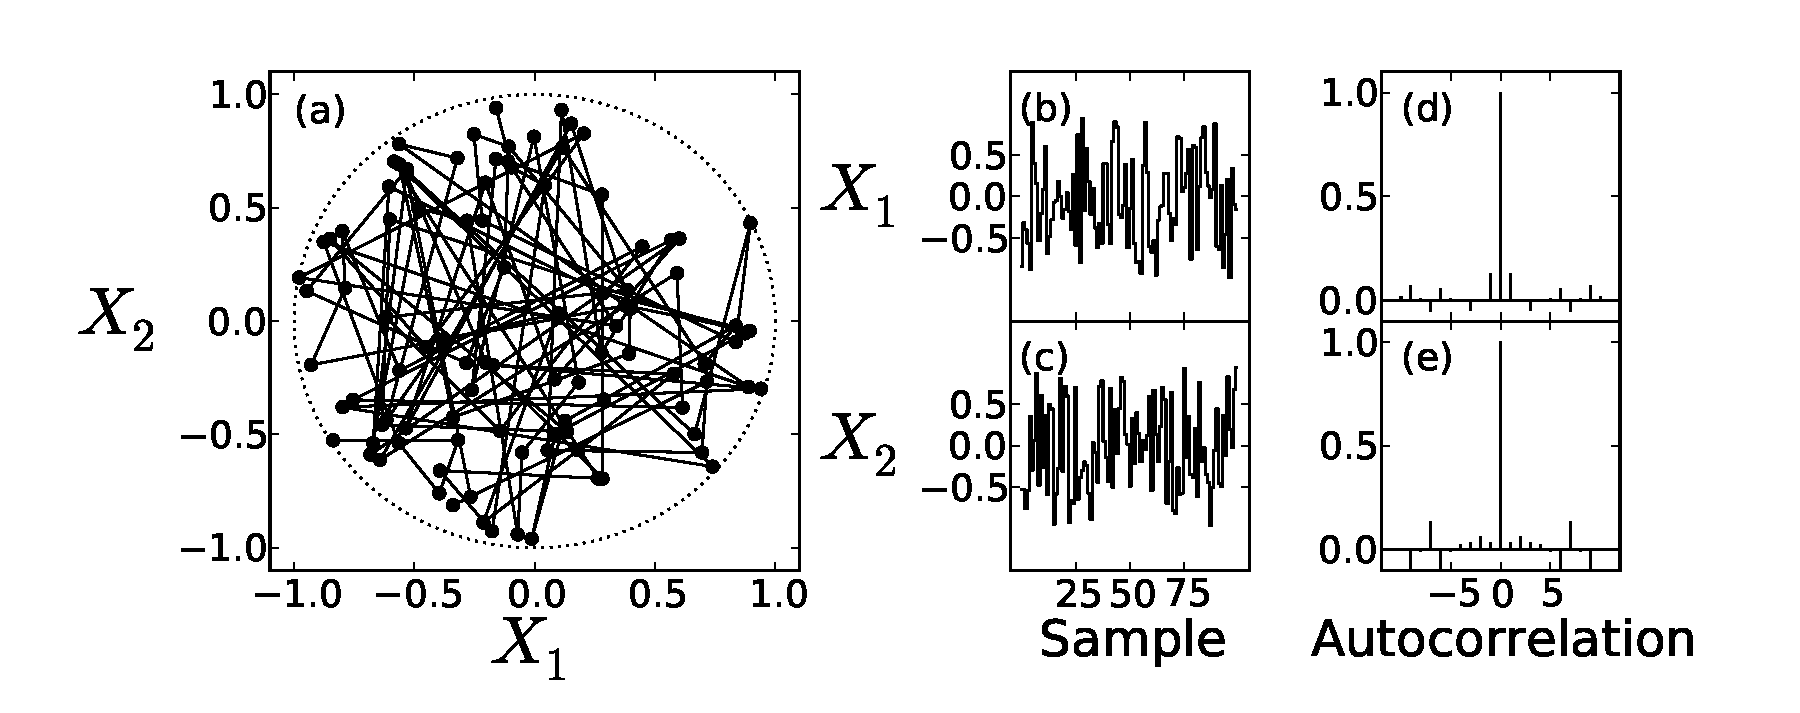
\includegraphics[width=\textwidth]{gibbs-ball.pdf}
\caption{The results of drawing 100 samples from a ball in two
  dimensions with MCMC using the Gibbs step method.  Although each
  sample is dependent on the previous samples, this dependence quickly
  decays, as shown by the plotting the autocorrelation function of
  $X_1(t)$ and $X_2(t)$ in panels (d) and (e).}
\label{gibbs-ball}
\end{center}
\end{figure}


To see that the uniform distribution of the chain is stationary
requires a small calculation.  What is the probability density of a
point $x \in \bbR^n$ after a single step of the chain?  If
$\dens(X_i=x) = \frac{1}{Z}$ for all $x$, with the notation
$\ell_d = \sqrt{1-\sum_{j \neq d} x_j^2}$,
\begin{align*}
\dens(X_{i+1}=x) &= \int\int\cdots\int \dens(X_{i+1}=x|X_i=x') \dens(X_i=x')\d x'_1 \d x'_2 \cdots \d x'_n\\
&=\sum_{d=1}^n \int \dens\left(X_{i+1}=x | X_i = (x_1, \ldots, x'_d, \ldots, x_n)\right)\\
&\qquad\qquad\qquad\qquad\times \dens\left(X_i = (x_1, \ldots, x'_d, \ldots, x_n)\right)\d x'_d\\
&=\sum_{d=1}^n \int_{-\ell_j}^{\ell_j} \frac{1}{n} \frac{1}{2\ell_d} \frac{1}{Z} \d x'_d\\
&=\frac{1}{Z}.
\end{align*}

Implementing each step of the chain is simple in this case, requires
only a way to choose numbers uniformly from the interval $[0,1]$.  This
is \emph{not} simple, but it a basic primitave that randomized
computation relies on; I use the Mersenne Twister pseudorandom number
generator, a well-tested standard.\cite{TK M. Matsumoto and T. Nishimura,
  “Mersenne Twister: A 623-dimensionally equidistributed uniform
  pseudorandom number generator”, ACM Transactions on Modeling and
  Computer Simulation Vol. 8, No. 1, January pp.3-30 1998.}
To generate $X_{i+1}$ from $X_i$, the following suffices:
\begin{itemize}
\item Choose dimesion $d_i \in [n]$ uniformly at random.
\item Choose sign $s_i \in \{-1, 1\}$ uniformly at random.
\item Choose fraction $f_i \in [0,1]$ uniformly at random.
\item Set $X_{i+1}$ equal to $X_i$ for all coordinates besides $d_i$ and let
\begin{align*}
X_{i+1}(d_i) &= s_i f_i \sqrt{1 - \sum_{j\neq d_i} x_j^2}
\end{align*}
\end{itemize}

An elegant proof that this chain rapidly converges to its stationary
distribution follows the coupling method.\cite{Torgey Lindval The
  Coupling Method} Here the goal is to design a joint distribution on
two copies of the Markov chain $(X, Y)$, so that the marginal
distribution of each copy is the same as the distribution above, and
then show that if chain $(X_0, X_1, \ldots)$ starts from an arbitrary
point with non-zero probability density $X_0$, and chain $(Y_0, Y_1,
\ldots)$ starts from the stationary distribution, then the expected
distance between $X_i$ and $Y_i$ tends quickly to zero as a function
of $i$.  If $\E[\|X_i - Y_i\|] \leq \e$ then for any statistic of
interest of $Y_i$, I can quantify the error when approximating it with
$X_i$, the value that comes out of my computation.

The attainable bound on the expected distance between $X_i$ and $Y_i$
depends critically on the joint distribution, or coupling.  One simple
approach is to choose the same dimension to alter in both chains,
choose the same direction to alter it, and then choose the same
fraction of the maximum allowable distance along this ray for both
chains.  In other words, to generate $(X_{i+1}, Y_{i+1})$:
\begin{itemize}
\item Choose dimesion $d_i \in [n]$ uniformly at random.
\item Choose sign $s_i \in \{-1, 1\}$ uniformly at random.
\item Choose fraction $f_i \in [0,1]$ uniformly at random.
\item Set $X_{i+1}$ and $Y_{i+1}$ equal to $X_i$ and $Y_i$ for all coordinates besides $d_i$ and let
\begin{align*}
X_{i+1}(d_i) &= s_i f_i \sqrt{1 - \sum_{j\neq d_i} x_j^2}\\
Y_{i+1}(d_i) &= s_i f_i \sqrt{1 - \sum_{j\neq d_i} y_j^2}.
\end{align*}
\end{itemize}

The marginal distributions $\dens(X_{i+1}=x|X_i)$ and
$\dens(Y_{i+1}=x|Y_i)$ are both equal to the chain above, and an
exercise in geometry shows that the distance between $X_i$ and $Y_i$
decreases in expectation with each step of the chain. Calculation TK.

\section{The Metropolis-Hastings step method}
As mentioned above, my approach to parameter estimation with MCMC does
\emph{not} rely on deriving Gibbs step methods, which are often much
more involved that the simple example in the previous section.  I rely
heavily on the Metropolis-Hastings (MH) step method, and an adaptive
variant thereof.

In the context of Bayesian statistics, the MH
algorithm is a technique used to sample from the posterior
distribution when the posterior distribution cannot be easily sampled
from directly. The algorithm generates the next position of its random walk
in two steps: first it makes a proposal by choosing from a proposal
probability distribution, which depends on the current value of the
walk. Then it accepts or rejects this proposal with a probability
carefully designed to yield the desired stationary distribution.

In the example from the previous section, uniform sampling from the
unit ball, the proposal distribution could be a normal distribution centered at the current value, for example
\[
P_i \sim \Normal\left(X_i, \Sigma^2\right).
\]
The MH rejection rule is based on the quantity $p_i =
\min\left(1, \frac{\dens(P_i)\dens'(P_i|X_i)}{\dens(X_i)\dens'(X_i|P_i)}\right)$, where
$\dens(\cdot)$ is the posterior probability density for value $x$, and
$\dens'(p, x)$ is the probability density of proposing $p$ when the
chain has value $x$.  The rejection rule is the following:
\[
X_{i+1} = \begin{cases}
P_i, &\quad\text{with probability } p_i;\\
X_i, &\quad\text{with probability } 1-p_i.
\end{cases}
\]
This simplifies considerable when sampling from the unit ball with the
symmetric proposal distribution above, to simply
\[
X_{i+1} = \begin{cases}
P_i , &\quad\text{if }\|P_i\| \leq 1;\\
X_i, &\quad\text{otherwise}.
\end{cases}
\]

Making the example from the previous section only a little bit more
complicated demonstrates both the utility and the challenges of the MH
step method for MCMC.  Instead of sampling from the unit ball, now I
will consider sampling uniformly from an ellipsiod in $n$ dimensions,
$\{x\in \bbR^n : x^T \Lambda x \leq 1\}$.  In this case, the Gibbs
step method requires solving a system of equations at each step to
determine the limits of the ellipse along the selected dimension.  The
MH step method requires only testing if the proposed point is in the
ellipse.  On the other hand, the Gibbs step method always moves to a
new point in the sample space, while MH sometimes rejects the proposal
and stays at the same point for multiple steps.  In either case, if
the ellipse is long and skinny, it will slow the chain.  The Gibbs
steps will not move very far much of the time, while the MH steps will
often not move at all.

When $n=2$, it is possible to visualize this example in two
dimensions, and Figure~\ref{metropolis-ball} shows the results for an
ellipse with width three times its height.

\begin{figure}[ht]
\begin{center}
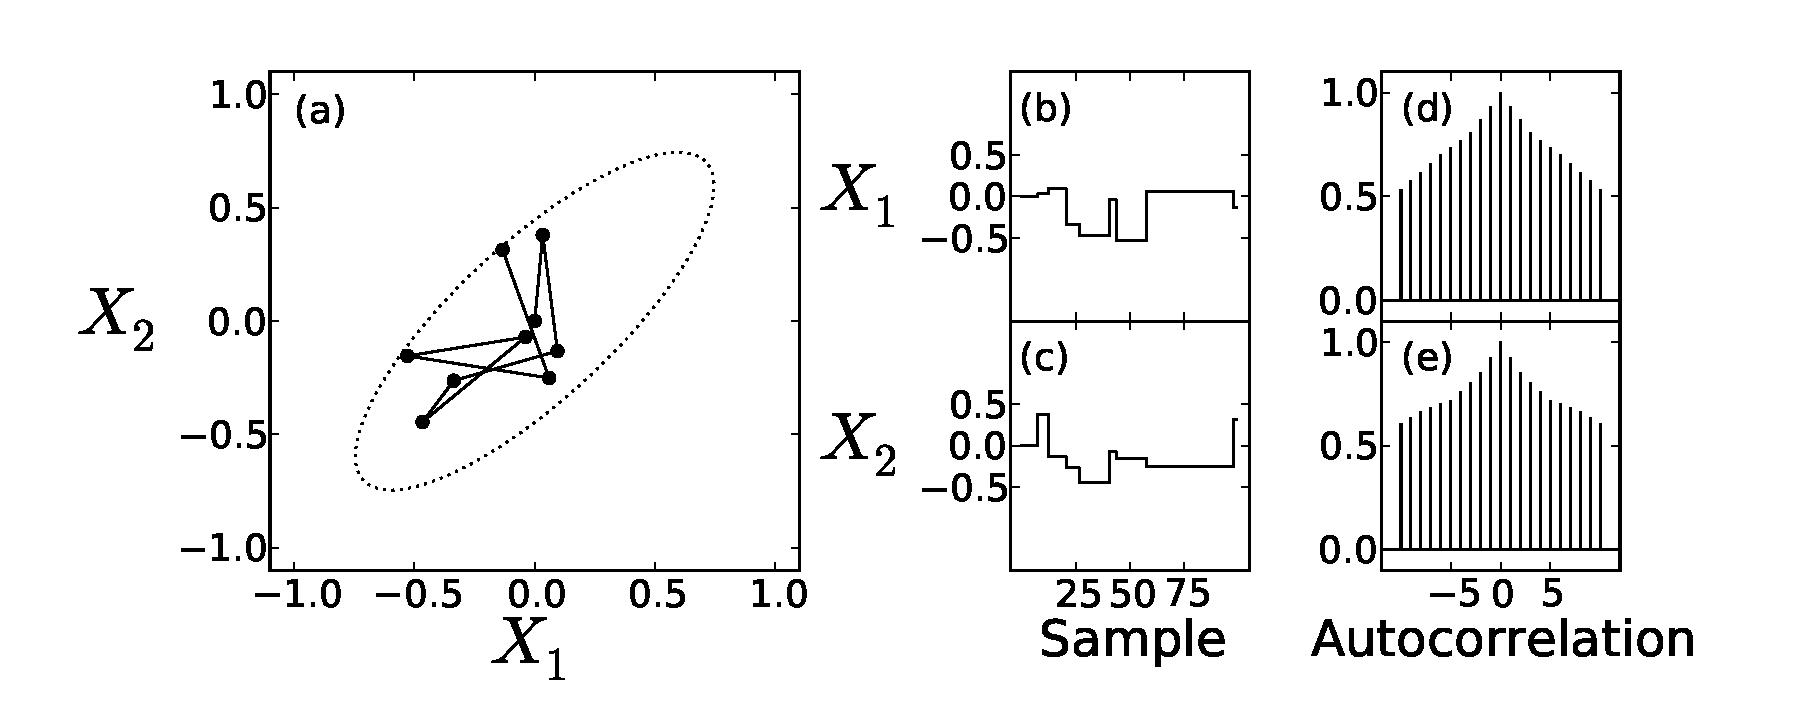
\includegraphics[width=\textwidth]{metropolis-ball.pdf}
\caption{The results of drawing 100 samples from an ellipse in two
  dimensions with MCMC using the MH step method.  Each sample is
  dependent on the previous samples, and because of the shape of the
  ellipse, the MH proposals are often infeasible, so the dependence
  does not decay rapidly, as shown by the plotting the autocorrelation
  function of $X_1(t)$ and $X_2(t)$ in panels (d) and (e).}
\label{metropolis-ball}
\end{center}
\end{figure}


\section{The Adaptive Metropolis step method}
The Adaptive Metropolis (AM) step method extends the
Metropolis-Hastings step method by adaptively adjusting the
variance-covariance matrix for the proposal distribution based on the
acceptance rate of the proposals.\cite{Harrio_paper_cited_in_PyMC}
Because the proposal acceptance rate is so important to algorithmic
efficiency, a long line of research has considered adaptive approaches
to proposal distribution selection.\cite{refs_from_harrio_and_others}

One popular adaptive approach is to use a simplified version of the MH
step method above (often called the Metropolis step method), where a
proposal is generated at each step
\[
P_i \sim \Normal\left(X_i, \Sigma^2_i\right),
\]
and then accepted or rejected with probability $p_i = \min\left(1,
\frac{\dens(P_i)}{\dens(X_i)}\right)$.  This is a simplification of
the MH step method, because the terms about the transition probability
are not included in the proposal acceptance probability.  But it has a
subtle complexification of the MH step method as well, because the
proposal distribution covariance matrix $\Sigma_i$ is now changing
as the chain progresses.  The goal is to change it in a way that
adapts to the distribution it is being used to sample from.

The adaptive values of $\Sigma_i$ that I have used follow those
implemented in the PyMC software package,\cite{Patil_PyMC_2010}
\[
\Sigma_i = \begin{cases}
\Sigma_0, &\qquad i \leq i_0;\\
s_n \left(\operatorname{cov}(X_0, \ldots, X_i) + \e I_n\right), &\qquad i > i_0.
\end{cases}
\]

The initial value for the covariance matrix, $\Sigma_0$, has a large
influence on the burn-in time required, and I will return to it below.
For the additional parameters, I have used the PyMC default values,
where in a $n$-dimensional sample space, I have $s_n = (2.4)^2/n$, $\e
= 10^{-5}$, and $I_n$ the $n$-dimensional identity matrix.

For additional computational speedup, I have followed the PyMC
modification of the original AM step and only updated $\Sigma_i$ every
$100$ or $1000$ steps.  Furthermore, if few proposals are
ever accepted, then I decrease the variance of the
proposal distribution by a constant faction.

When $n=2$, the results of this step method can be visualized in two
dimensions, and Figure~\ref{am-ball} shows the results of the AM
stepper after $20000$ iterations have been run to allow the covariance
matrix to adapt to the posterior distribution.

\begin{figure}[ht]
\begin{center}
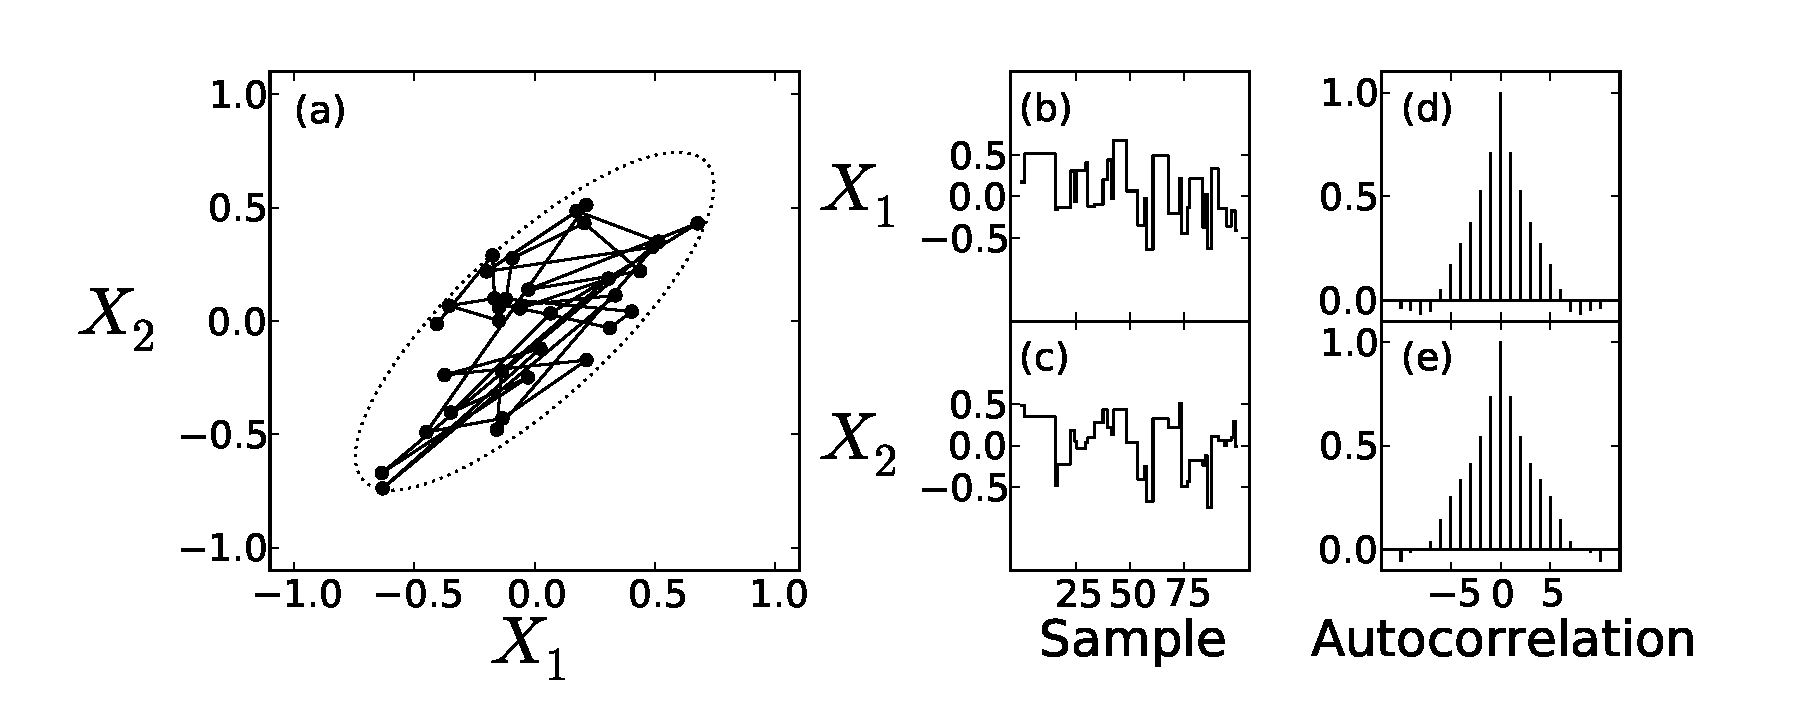
\includegraphics[width=\textwidth]{am-ball-2.pdf}
\caption{The results of drawing 100 samples from an ellipse in two
  dimensions with MCMC using the AM step method, after 20000
  iterations of ``burn-in''.  Each sample is dependent on the previous
  samples, but after a period of exporation, the AM proposals become
  aligned with the axes of the ellipse, and the dependence decays more
  rapidly than in the MH approach from Figure~\ref{metropolis-ball}.}
\label{am-ball}
\end{center}
\end{figure}

\section{Convergence of the MCMC algorithm}

The chief pitfall of the MCMC algorithm is nonconvergence.  A line of
theoretical research in computer science is devoted to identifying
classes of distributions and classes of step methods for while MCMC
can be proven to converge rapidly.\cite{TCS_refs_on_convergence}
Unfortunately, this work has recently developed strong evidence
against the possibility of automatically detecting convergence of MCMC
in general.\cite{Trevisan_et_al_MCMC_convergence} This work has
developed largely separately from the Bayesian computing literature,
where posterior estimates generated by MCMC sampling are used
frequently in important settings.\cite{PK,Eco,Stats,Astro_examples} In
the applied statistical literature, MCMC is too convenient not to be
used, and since nonconvergence is such an important pitfall, a vast
array of heuristic checks for convergence have developed over the
years.\cite{key_examples_of_convergence_heuristics} A recent survey
compared and contrasted many of
these.\cite{survey_of_convergence_techniques}

Essential to using MCMC for statistical estimation is reproducibility,
and here is where nonconvergence wreaks its havoc.  MCMC computation
is randomized computation, meaning the same algorithm run on the same
data twice will give slightly different answers.  This is fine, as
long as the variation between successive runs can be controlled.  When
MCMC has not converged, the difference between two runs cannot be
predicted, which means the results will not be reproducible.  This
must be avoided for MCMC computation to be useful.

One heuristic to identify nonconvergence that has been particularly
useful in my work is to visually inspect the autocorrelation plot for
each dimension of the sample space.  This autocorrelation function is defined by
\[
\text{acf}(\tau) = \frac{\E\left((X_i - \mu)(X_{i+\tau} - \mu)\right)}{\sigma^2},
\]
where $\mu$ and $\sigma$ are the mean and standard deviation of the
posterior distribution.  The autocorrelation plot for independent
samples is a delta function, and the rate of decay of the
autocorrelation plot gives some indication of how close the samples
are to being uncorrelated.  The panels (d) and (e) from the
Figures~\ref{gibbs-ball}, \ref{metropolis-ball}, and \ref{am-ball}
show autocorrelation plots in a provably rapidly mixing chain
(Figure~\ref{gibbs-ball}), in a clearly nonconvergent case
(Figure~\ref{metropolis-ball}), and in a marginal case that I would
run for longer to be sure (Figure~\ref{am-ball}).

There are three general approaches to improve the convergence of MCMC
computation. The first and simplest approach is to run the chain for
longer and thus take more samples.  In the long run, the algorithm
will succeed, and the only question is can the program run for long
enough in the time available for the analysis? The second approach is
to use a more appropriate step method, for example by using AM steps
instead of the MH steps in the ellipse example above.  Other more
complicated step methods can also be used, and the development of new
and improved step methods is an active area of research.  The third
approach is to use better initial values for the MCMC, which includes
both starting from a likely point in the posterior distribution and,
in the case of AM and other advanced step methods, initializing the
step method parameters wisely as well.

The wise selection of initial values is the topic of the next section.

\section{Initial values for MCMC}
Past research has found that the choice of initial values for MCMC can
dramatically affect the time necessary for convergence.  In
theoretical work, TK summary of ``warm-start''
results.\cite{Hit_and_run_papers} In practice, a number of different
methods have been proposed for generating initial values for MCMC
samplers.\cite{Gelman_Rubin_1992a,
  Applegate_Kannan_Polson_1990,Jennison_1993,Brooks_Gelman,Brooks_1998}
The simplest approach is to choose initial values from the prior
distribution.  In my experience, this is not as stable as choosing
initial values based on the results of a local optimization procedure
that finds an initial value approximately maximizing the posterior
distribution.

I have used a combination of coordinate descent and Powell's method to
find a local maximum of the posterior distribution which I then used
as the initial values for
MCMC.\cite{Tseng_Convergence_2001,Powell_An_1964} In addition to
finding a good initial point in the sample space, it is also helpful
to find good initial values for the covariance matrices of the AM step
methods.  To do this, I use the normal approximation at the maximum
posterior, which seems to work well in practice.


\section{Empirical Bayesian priors to borrow strength between regions}
\label{empirical-priors}

When making estimates for all 21 geographic regions in the Global
Burden of Disease (GBD) 2010 Study, the available data is often very
sparse.  I have often used an approach to borrow strength between
regions that in described in this section.  It is a two-stage approach
that can be characterized as an empirical Bayesian technique.

The mechanics of this approach are simple.  First, I fit a model to
the available data at the global level.  Depending on the data
available, this is often either an inconsistent model, using the
random effect age-integrating negative-binomial spline model from
Chapters~\ref{theory-age_pattern_model} to
\ref{theory-covariate_modeling}, or a consistent model linking random
effect age-integrating negative-binomial spline models for different
epidemiological parameters through the system of differential
equations in Chapter~\ref{sys-dynamics}.  This model is used to make
estimates for all regions of the world.

The second stage of the empirical Bayes approach is to use the first
stage predictions for a region as priors, and to fit the model again,
now including the empirical priors, with only the data relevant to a
particular region, sex, and year.


\section{Future directions for research}

MCMC has been an enabler for this approach.  Without free/libre
open-source software for implementing AM/MCMC this project would not
have been possible.  But it is not the only approach.  Message passing
algorithms have proven themselves quite successful in related
computational challenges.\cite{TK} Nonlinear optimization is another
promising approach, especially combined with bootstrap method for
estimating uncertainty.\cite{dm4_paper} Finally, there are a number of
recent developments in MCMC methods as well, includeing population
monte carlo, the t-walk, and Hamiltonian MC, all of which could yield
faster convergence.\cite{several_papers_on_this}


